% ---- ETD Document Class and Useful Packages ---- %
\documentclass{ucetd}
\usepackage{subfigure,epsfig,amsfonts}
\usepackage{natbib}
\usepackage{amsmath}
\usepackage{amssymb}
\usepackage{amsthm}
\usepackage[toc,page]{appendix}
\usepackage[labelfont=bf]{caption}
\usepackage{rotating}
\usepackage[dvipsnames]{xcolor}
\usepackage{url}
\usepackage{bm}
\usepackage{bbm}

%% Use these commands to set biographic information for the title page:
\title{Phase transitions of DNA-protein condensates during the immune response}
\author{Clayton W. Seitz}
\department{Department of Physics}
\division{Physical Sciences}
\degree{Doctor of Philosophy}
\date{Spring 20XX}

%% Use these commands to set a dedication and epigraph text

\epigraph{Epigraph}



\begin{document}
%% Basic setup commands
% If you don't want a title page comment out the next line and uncomment the line after it:
\maketitle
%\omittitle

% These lines can be commented out to disable the copyright/dedication/epigraph pages
\makecopyright
%\makededication


%% Make the various tables of contents
\tableofcontents
%\listoffigures
%\listoftables

%\acknowledgments
% Enter Acknowledgements here

\abstract

Eukaryotic transcription is episodic, consisting of a series of transcriptional bursts, Bursty transcriptional dynamics are well-exemplified by the transient expression of pro-inflammatory guanylate binding proteins (GBPs) - a group interferon-inducible GTPases that restrict the replication of intracellular pathogens [XXX]. Classical models of gene regulation explain transcriptional bursts by invoking stochastic binding and unbinding of transcription factors, RNA polymerase and mediator proteins at enhancer or promoter sequences. However, more recent studies have pointed towards a more cooperative picture of transcriptional control where phase-separated aggregates of DNA, RNA, and proteins form higher-order structures to control gene expression. For example, both chromatin immunoprecipitation and super resolution imaging have captured the phase separation of super-enhancer-binding proteins MED1 and BRD4 in transcriptional condensates at the \textit{Essrb} genomic locus [XXX]. Furthermore, fluorescence microscopy techniques have colocalized MED1 and BRD4 with the GBP gene cluster alongside a reduction in the degree of disorder of 3D chromatin structure in murine macrophages after infection with \textit{Mycobacterium tuberculosis}. Taken together, these results suggest that phase separation may play a role in the reorganization of chromatin structure during trancriptional control of innate immune response genes [XXX]. Here, we hypothesize that phase separation reduces the entropy of chromatin structure in order to induce bursty gene expression. Using single molecule localization microscopy (SMLM) to obtain super-resolution images of the H2B protein, we intend to demonstrate simultaneous (i) loss of disorder in chromatin structure (ii) formation of transcriptional condensates containing MED1 and BRD4 and (iii) non-Poissonian gene expression. The following sections discuss recent the biological evidence in more detail and summarize the single molecule microscopy techniques and biophysical models we employ to study the interactions between transcriptional condensates and the chromatin scaffold.

\clearpage

\mainmatter

\chapter{Literature Review and Theoretical Foundations}

\chapter{Single molecule localization microscopy}


This principle of SMLM is at the same time one of its primary limitations: the need for sparse activation leads to long acquisition times and expensive autofocusing equipment to actively correct for sample drift. This results in low throughput, poor time resolution when imaging dynamic processes, low labeling densities and a reduced choice of fluorophores. In addition, the need for sparse activation requires laborious optimization of dSTORM buffers containing oxygen scavenging systems and/or oxygen purging techniques. In response to these problems, a host software tools for SMLM have emerged, which permit the acquisition of emitters at higher densities. (Speiser 2021). In the multi-emitter setting, PSFs are no longer well-separated but may overlap, adding additional uncertainty into the localization process. Existing algorithms have explicitly modeled the point spread function as a mixture of single molecule PSFs or have utilized deep learning-based tools to estimate the parameters of each PSF embedded in the mixture.  

Due to overlap, conventional detection strategies may undercount the emitters in a local neighborhood in some frames, localization uncertainty can increase for overlapping emitters, and some localizations may be missed entirely. These complications make conventional detection strategies inappropriate for reconstruction of super-resolution images from time-series. Perhaps most importantly, overlapping emitters can result in additional localization uncertainty, rendering discernment between the arrival of a new particle and a poorly localized existing one difficult. This issue poses a major bottleneck to super-resolution imaging acqusitions. Additional uncertainty can be partially alleviated by using pairwise or higher-order temporal correlations within a pixel neighborhood to deconvolve individual emitters. A similar idea is employed in super-resolution optical fluctuation imaging (SOFI) - a post-processing technique that uses image cumulants to deconvolve emitters. 

Existing correlation-based techniques have been succesful in reaching XXX resolution; however, they are not easily integrated into a Bayesian workflow. The Bayesian philosophy is an important one, as it guards against overfitting of poorly designed models to experimental observations. Furthermore, combining Bayesian inference methods and information theoretic ones, we can begin to ask questions like: can we (even in principle) reduce our uncertainty in localization parameters using time-series data? That is, does a time series $\vec{H}$ carry any \emph{information} that an estimator $\mathcal{E}$ can use to infer the number of fluorophores and their coordinates more precisely? The success of optical fluctuation methods suggests they can; however, the information content of time-series on particle localization and methods for its efficient extraction remain largely unexplored. 

\section{A generative model for single molecule localization microscopy}

Most detectors used for imaging have many elements (pixels) so that we can record an image projected onto the detector by a system of lenses. In fluorescence imaging, this is usually a relay consisting of an objective lens and a tube lens to focus the image onto the camera. Due to diffraction, any point emitter, such as a single fluorescent molecule, will be registered as a diffraction limited spot. The profile of that spot is often described as a Gaussian point spread function

\begin{equation}
\mathrm{G}(x,y) = \frac{1}{2\pi\sigma^{2}}e^{-\frac{(x-x_{0})^{2}+(y-y_{0})^{2}}{2\sigma^{2}}} + B_0
\end{equation}

\begin{figure}
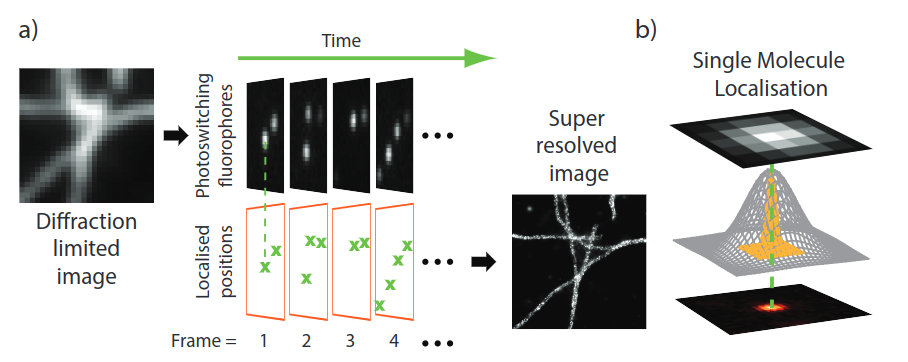
\includegraphics[scale=0.525]{Figure-0.png}
\end{figure}

Modern cameras used in light microscopy, such as scientific complementary metal oxide semiconductor (sCMOS) cameras, are powered by the photoelectric effect. Electrons within each pixel, called photoelectrons, absorb enough energy from incoming photons to be promoted to the conduction band to give electrical current which can be detected. Integration of photoelectrons during the exposure time results in a monochrome image captured by a camera. The image of a single point particle, such as a fluorescent molecule, can be thought of as two-dimensional histogram of photon arrivals and a discretized form of the classical intensity profile $\mathrm{G}(x,y)$. The value at a pixel approaches an integral of this density over the pixel:

\begin{equation}
\mu_{k} = I_{0}\lambda_{k} = I_{0}\int_{\mathrm{pixel}} G(x,y)dxdy
\end{equation}

where $I_{0} = \eta N_{0}\Delta$. The parameter $\eta$ is the quantum efficiency and $\Delta$ is the exposure time. $N_{0}$ represents the number of photons emitted per unit time, which may be itself a Poisson random variable; however, this is inconsequential since it is a fixed value for a single image of a fluorescent molecule. If the background signal is not negligible, then we can generalize (2.2) above to

\begin{equation}
\mu_{k} = \eta\Delta\left(N_{0}\lambda_{k} + B_{0}\right)
\end{equation}

where $B_{0}$ is the rate that background photons arrive at pixel $k$. The value of the integral $\lambda_{k}$ at a pixel $k$ defines the fraction of $N_{0}$ photons that arrive at pixel $k$ during the camera exposure. Since the 2D Gaussian in (1.1) has cylindrical symmetry, it is separable, and we can write

\begin{align*}
\lambda_{k} &= \frac{1}{2\pi\sigma^{2}}\left(\int_{x_{k}}^{x_{k+1}}e^{-\frac{(x-x_{0})^{2}}{2\sigma^{2}}}dx\right)\left(\int_{y_{k}}^{y_{k+1}}e^{-\frac{(y-y_{0})^{2}}{2\sigma^{2}}}dy\right)
\end{align*}


We can then express the Gaussian integrals over a pixel by making use of the following property of the error function

\begin{equation*}
\frac{1}{\sqrt{2\pi}\sigma}\int_{a}^{b} e^{\frac{-(x-\mu)^{2}}{2\sigma^{2}}} = \frac{1}{2}\left(\mathrm{erf}\left(\frac{b-\mu}{\sqrt{2}\sigma}\right) -\mathrm{erf}\left(\frac{a-\mu}{\sqrt{2}\sigma}\right)\right)
\end{equation*}

Now, suppose the particle is known to be located at $(x_{0},y_{0})$ and some square pixel $k$ is centered on coordinates $(x,y)$ and has a width $a$. Then $\lambda_{k}$ at this pixel is

\begin{equation}
\lambda_{k}(x,y) = \lambda_{x}(x)\lambda_{y}(y)
\end{equation}

where

\begin{align*}
\lambda_{x}(x) &= \frac{1}{2}\left(\mathrm{erf}\left(\frac{x+a/2-x_{0}}{\sqrt{2}\sigma}\right) -\mathrm{erf}\left(\frac{x-a/2-x_{0}}{\sqrt{2}\sigma}\right)\right)\\
\lambda_{y}(y) &= \frac{1}{2}\left(\mathrm{erf}\left(\frac{y+a/2-y_{0}}{\sqrt{2}\sigma}\right) -\mathrm{erf}\left(\frac{y-y/2-y_{0}}{\sqrt{2}\sigma}\right)\right)
\end{align*}

We are now prepared to write the shot-noise limited signal, which is a vector with units of phototelectrons

\begin{equation}
\vec{S} = \left[\mathrm{Poisson}(\mu_{1}), \mathrm{Poisson}(\mu_{2}), ..., \mathrm{Poisson}(\mu_{N})\right]
\end{equation}


However this noise model is incomplete, because detectors often suffer from dark noise, which may refer to readout noise or dark current, and contributes to a nonzero signal even in the absence of incident light. Dark current is due to statistical fluctuations in the photoelectron count due to thermal fluctuations. Readout noise is introduced by the amplifier circuit during the coversion of photoelectron charge to a voltage. Here, we use the Hamamatsu ORCA v3 CMOS camera, which is air cooled to -10C and has very low dark current - around 0.06 electrons/pixel/second - and can therefore be safely ignored for exposure times on the order of milliseconds. Readout noise has been often neglected in localization algorithms because its presence in EMCCD cameras is small enough that it can be ignored within the tolerances of the localization precision. In the case of sCMOS cameras, however, the readout noise of each pixel is significantly higher and, in addition, every pixel has its own noise and gain characteristic sometimes with dramatic pixel-to-pixel variations.

It is important to note that we cannot measure the contribution by readout noise before amplification and therefore it must be expressed in units of $\mathrm{ADU}$. This is in contrast to $\vec{S}$, which can be expressed in units of photoelectrons, because these statistical fluctuations can be predicted to be Poisson by quantum mechanics. Furthermore, the number of photoelectrons $S_{k}$ is  multiplied by a gain factor $g_{k}$ which has units of $[\mathrm{ADU}/e^{-}]$, which generally must be measured for each pixel. Here, we will always assume that readout noise per pixel $\xi_{k}$ is Gaussian with some pixel-specific offset $o_{k}$ and variance $\sigma_{k}^{2}$. We will also assume that gain factors and pixel noise characteristics are constants and do not scale with the signal level $S_{k}$. Therefore our measurement, in units of ADU, is: 

\begin{equation}
\vec{H} = \vec{S} + \vec{\xi}
\end{equation}

What we are after is the joint distribution $P(\vec{H})$. A fundamental result in probability theory is that the distribution of $H_{k}$ is the convolution of the distributions of $S_{k}$ and $\xi_{k}$,

\begin{align}
P(H_{k}|\theta) &= P(S_{k})\circledast P(\xi_{k})\\
&= A\sum_{q=0}^{\infty} \frac{1}{q!}e^{-\mu_{k}}\mu_{k}^{q}\frac{1}{\sqrt{2\pi}\sigma_{k}}e^{-\frac{(H_{k}-g_{k}q-o_{k})}{2\sigma_{k}^{2}}}
\end{align}

where $P(\xi_{k}) = \mathcal{N}(o_{k},\sigma_{k}^{2})$ and $P(S_{k}) = \mathrm{Poisson}(g_{k}\mu_{k})$. In practice, this expression is difficult to work with, so we look for an approximation. Notice that 

\begin{align*}
\xi_{k} - o_{k} + \sigma_{k}^{2} \sim \mathcal{N}(\sigma_{k}^{2},\sigma_{k}^{2}) \approx \mathrm{Poisson}(\sigma_{k}^{2})
\end{align*}

Since $H_{k} = S_{k} + \xi_{k}$, we transform $H_{k}' = H_{k} - o_{k} + \sigma_{k}^{2}$, which is distributed according to 

\begin{align*}
H_{k}' \sim \mathrm{Poisson}(\mu_{k}')
\end{align*}

where $\mu_{k}' = g_{k}\mu_{k} + \sigma_{k}^{2}$. This result can be seen from the fact the the convolution of two Poisson distributions is also Poisson. Under this approximation, the model negative log-likelihood is

\begin{align}
\ell(\vec{H}) &= -\log \prod_{k} \frac{e^{-\left(\mu_{k}'\right)}\left(\mu_{k}'\right)^{n_{k}}}{n_{k}!}\\
&= \sum_{k}  \log n_{k}! + \mu_{k}' - n_{k}\log\left(\mu_{k}'\right)
\end{align}


\subsection{The multi-emitter regime}

The multi-emitter case is a straightforward extension of the single emitter case. Since noise is signal-independent, we write


\begin{equation}
\vec{H} = \sum_{k=1}^{K}\vec{S}_{k} + \vec{\xi}
\end{equation}

Since the sum of independent Poisson variables is itself a Poisson variable with a rate equal to the sum over rates of the individual processes, we can immediately write

\begin{align*}
H_{k}' &\sim \mathrm{Poisson}(\mu_{k}')\\
\mu_{k}' &= g_{k}\eta\Delta\left(\sum_{j}N_{j}\lambda_{\theta_{j}}(x_{k},y_{k}) + B_{0}\right)+ \sigma_{k}^{2}
\end{align*}

and of course we still have a negative log-likelihood that is identical to (2.9).

\subsection{The Cramer-Rao lower bound}

A general task in Bayesian inference is to determine $\theta$ from the data under the model $\mathcal{M}_{\theta}$. We may then ask - does the log-likelihood $\ell$ vary as we vary the parameters? If the likelihood is flat, all parameter sets are equally likely and the data does not appear to carry much information about the parameters. Moreover, if $\ell$ has a number of bumps or inflection points, then we expect that maybe some parameter sets are more likely that others. The ``bumpiness" of the likelihood surface is called the Fisher information - a fundmantal concept in information geometry. The Fisher information matrix $I(\theta)$ can be directly related to the curvature of the KL-Divergence over the parameter space

\begin{align*}
\nabla^2_{\theta'} D_{KL}[\ell(H|\theta) \parallel \ell(H|\theta')] 
&= - \nabla_{\theta'} \int \ell(H|\theta) \nabla_{\theta'}  \log \ell(H|\theta') \, dH \\ 
&= - \int \ell(H|\theta) \nabla^2_{\theta'}  \log \ell(H|\theta') \, dH \\
&= - \mathbb{E}_{\theta}[\nabla^2_{\theta'} \log \ell(H|\theta')] \\
&= I(\theta)
\end{align*}


We often call the Hessian matrix the \emph{score}. The Fisher information is the result of averaging the score over the parameter space. To be clear, the score is a function of the \emph{data}, not the parameters. It is a measure of sensitivity of the likelihood to changes in the parameters. Of course, the Fisher information matrix also depends on the parameterization chosen. Looking at (1.4), the likelihood is a hierarchical function that maps a vector space $\Theta$ to a vector space $\Lambda$ to a scalar value. Formally, we define $T: \Theta \rightarrow \Lambda$ and $W: \Lambda \rightarrow \mathbb{R}$. The parameter vector $(x_{0},y_{0},\sigma, N_{0})\in \Theta$, the Poisson rate vector $\vec{\lambda} \in \Lambda$ and $\ell \in \mathbb{R}$. To get the Hessian, we need the chain-rule for Hessian matrices.


\begin{align*}
\hat{H}_{(\ell,\theta)} = \hat{J}_{(\lambda,\theta)}^{T} \hat{H}_{(\ell,\lambda)} \hat{J}_{(\lambda,\theta)} + (J_{(\ell,\lambda)}\otimes I_{n})\hat{H}_{(\lambda,\theta)}
\end{align*}

In the second term of the equation, we have a Kronecker product between the Jacobian matrix of the likelihood with respect to the parameters of the hierarchical model ($J_{(L,\lambda)}$) and the $n\times n$ identity matrix ($I_n$), denoted as $J_{(L,\lambda)}\otimes I_n$. This Kronecker product gives a diagonal matrix where the elements along the diagonal are the elements of the vector $J_{(L,\lambda)}$.


\section{MAP estimation from SMLM time series}

We now address the problem of inferring photoswitching constants and fluorophore locations from SMLM time series $\bm{H}$. In the Bayesian framework, we write the posterior on $\Theta$ according to Bayes rule. We define the following hierarchical Bayesian model

\begin{align*}
\Theta &\sim P(\Theta)\\
S|\Theta &\sim P(S|\Theta)\\
\bm{H}|\Theta,S &\sim P(\bm{H}|\Theta,S)
\end{align*}

with the following posterior distribution

\begin{align*}
P(\Theta,S|\bm{H}) = \frac{P(\bm{H}|\Theta,S)P(S|\Theta)P(\Theta)}{P(\bm{H})}
\end{align*}

Let us first address the likelihood function. It is reasonable to propose that the joint distribution over a frame will factor into image neighborhoods due to locality. Therefore, we define the \emph{pixel assignment} $\bm{S}$ such that $\bm{S}(x,y)$ is assigned a label designating the fluorophore or combination of fluorophores collected photons were emitted by. The probability of an assignment given the particle locations is definite i.e., $P(S|\Theta) = \delta(S)$ where each pixel is attributed a \emph{labeling set}

\begin{equation*}
\bm{S}(x,y) =  \{\mathbbm{1}\left(\lambda_{n}(x,y) > \epsilon\right)\}_{n=1}^{N}
\end{equation*}
 
for some minimum rate tolerance $\epsilon << 1$. The neighborhood assignment $S$ can be absorbed into the parameter set and included as part of the inference problem. We can now see that the neighborhood $\bm{N}_{k} = \{H_{1},...,H_{N}\}$ per particle includes all pixels which detected photons from fluorophore $k$. When conditioned on $S$, the likelihood will factor into several smaller joint distributions. That is,

\begin{align*}
P(\bm{H}|\Theta,S) &= \prod_{k}P(\bm{N}_{k}|\Theta,S)
\end{align*}

The probability $P(\bm{N}_{k}|\Theta,S)$ can be computed using the forward-backward algorithm. However, that calculation will simplify considerably if we notice that the sequence $\bm{N}_{k}$ is only dependent on a small part of the hidden state.

\subsection{Neighborhood sequence probabilities depend only on a small partition of the hidden state}

Before using the forward-backward algorithm to compute the probability of a neighborhood sequence $P(\bm{N}_{k}|\Theta,S)$, we want to simplify the problem by removing the hidden state subspace that $\bm{N}_{k}$ is not dependent on. This property is given by the locality implied in $S$

\begin{align*}
P(\bm{N}_{k}|\Theta,S) &= \sum_{\bm{X}}P(\bm{N}_{k},\bm{X}|\Theta,S) \\
&= \sum_{\bm{X}}P(\bm{N}_{k}|\bm{X},\Theta,S)P(\bm{X}|\Theta,S)
\end{align*}


\begin{figure}
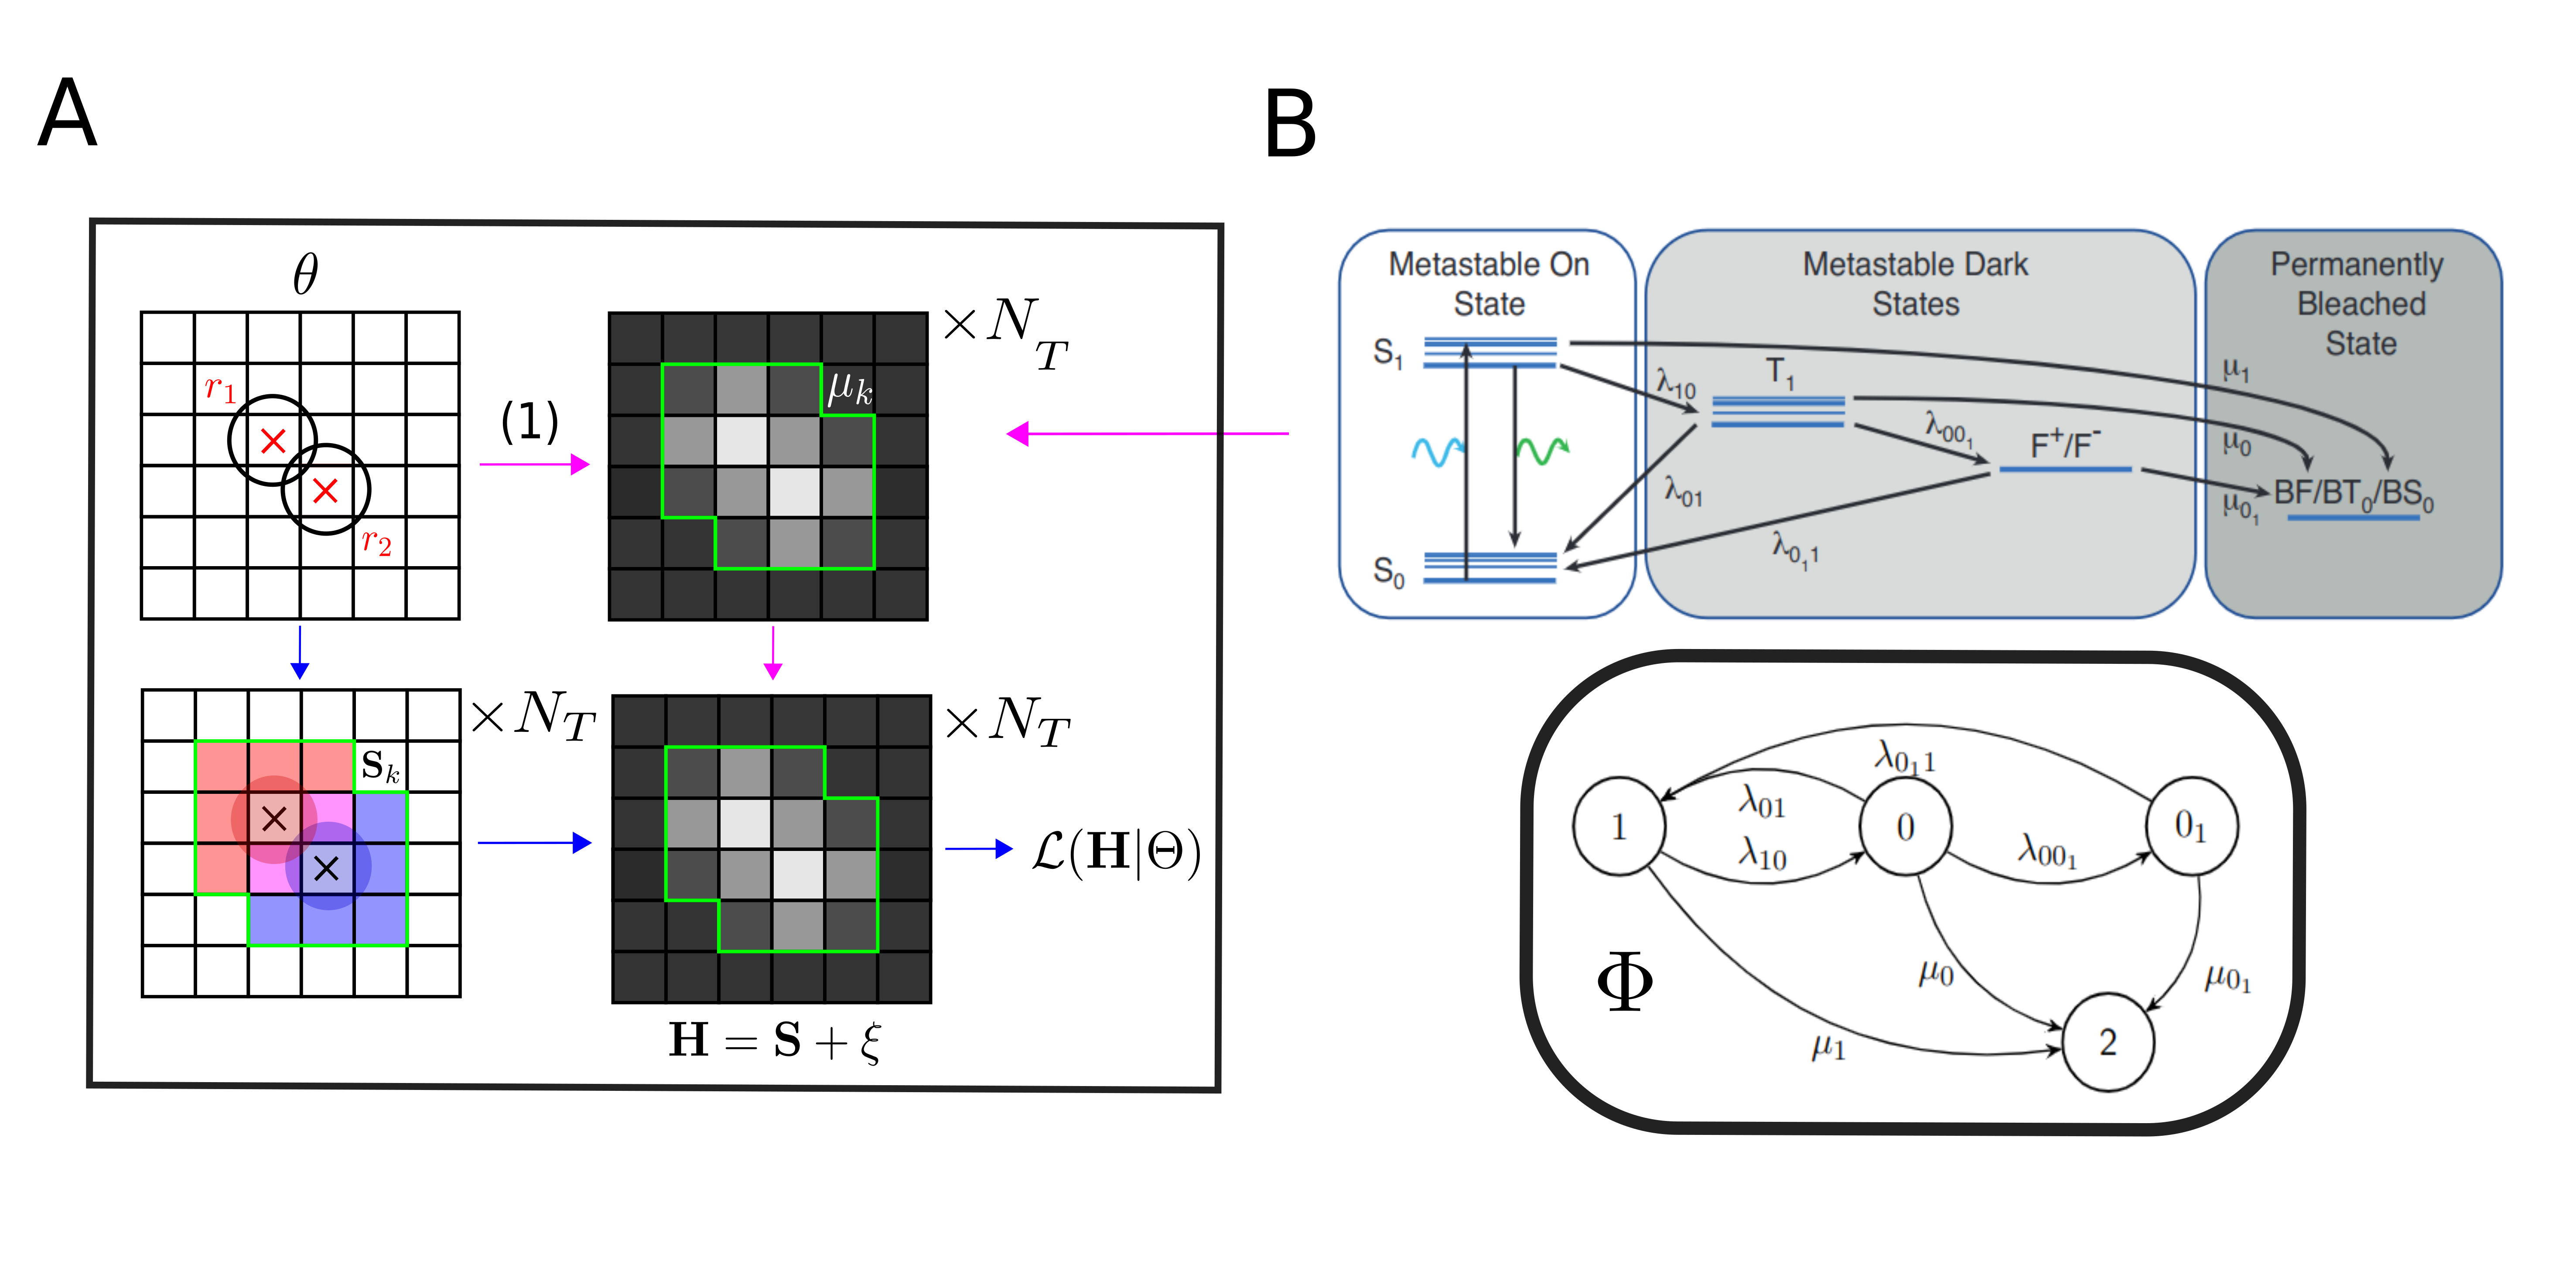
\includegraphics[scale=0.325]{Schematic.png}
\caption{(A) Generative path (violet) and likelihood computation (blue) for a single pixel neighborhood (outlined in green). During inference, the pixels are labeled according to which fluorophore(s) they count photons from, simplifying the likelihood computation. (B) Continuous-time Markov chain (CTMC) model used both for synthetic data generation (simulated via SSA), and inference of photoswitching kinetics with PSHMM module}
\end{figure}

We now leverage the conditional independence structure embedded in $S$. That is, $S$ implies that each neighborhood sequence  $\bm{N}_{k}$ depends only on a small subset of $\bm{X}$, so we can define $\bm{Y}$ as the partition of sequence $\bm{X}$ that it depends on and $\bm{Z}$ the partition it does not. This implies that $P(\bm{N}_{k}|\bm{X},\Theta,S) = P(\bm{N}_{k}|\bm{Y},\Theta,S)$. Therefore,

\begin{align*}
P(\bm{N}_{k}|\Theta,S) &= \sum_{\bm{Z}}\sum_{\bm{Y}}P(\bm{N}_{k}|\bm{Y},\bm{Z},\Theta)P(\bm{Y},\bm{Z}|\Theta)\\
&= \sum_{\bm{Z}}P(\bm{Z}|\Theta)\sum_{\bm{Y}}P(\bm{N}_{k}|\bm{Y},\bm{Z},\Theta)P(\bm{Y}|\bm{Z},\Theta)\\
&= \sum_{\bm{Y}}P(\bm{N}_{k}|\bm{Y},\Theta)P(\bm{Y}|\Theta)\\
\end{align*}

\subsection{The forward-backward algorithm}

Now that we have proven that we only need a small parition of the hidden state to compute the probability of a neighborhood sequence $P(\bm{N}_{k}|\Theta,S)$ we can move on to the forward-backward algorithm.

\section{Markovian photoswitching dynamics}

The true photo-switching behavior of the fluorophore is a continuous time stochastic phenomenon. However, an experimenter can only ever observe a discretized manifestation of this
by imaging the fluorophore in a sequence of frames. These frames are regarded as a set of
sequential exposures of the fluorophore and the observed discrete time signal indicates whether
the fluorophore has been observed in a particular frame. It is the continuous time process on
which we wish to draw inference based on the observed discrete-time process indicating whether
the fluorophore was observed in a frame. In this section we first present the continuous time
Markov model of the true (hidden) photo-switching behavior, and then derive the observed
discrete time signal, together with key results on its statistical properties.


We model the photoswitching behavior of a fluorophore as a continuous time Markov process. It is a stochastic process, which satisfies the Markov property

\begin{equation*}
P(X_{t}|X_{t-1}, X_{t-2}, ..., X_{t-N}) = P(X_{t}|X_{t-1})
\end{equation*}

We consider a general model for $X(t)$ that can accommodate the numerous mechanisms of photo-switching utilized in standard SMLM approaches such as (F)PALM and (d)STORM. Specifically, this model consists of a photon emitting (On) state $1$, $m+1$ non photon emitting (dark/temporary off) states $0_0$, $0_1$, $\ldots$, $0_m$, where $m \in \mathbb{Z}{\geq 0}$, and a photobleached (absorbing/permanently off) state $2$. In order to accommodate for the $m = 0$ case when we have a single dark state, we use the notational convention that state $0_0 \equiv 0$. The model, allows for transitions from state $1$ to the multiple dark states (from a photochemical perspective, these can include triplet, redox and quenched states). These dark states are typically accessed via the first dark state $0$ (reached as a result of inter-system crossing of the excited $S1$ electron to the triplet $T1$ state). Further dark states $0_{i+1}$, $i = 0, \ldots, m-1$, are accessible by previous dark states $0_i$ (by, for example, the successive additions of electrons forming radical anions (Van de Linde et al., 2010)). We allow the On state $1$ to be accessible by any dark state and we consider the most general model in which the absorption state $2$ is accessible from any combination of other states (Vogelsang et al., 2010; Van de Linde and Sauer, 2014; Ha and Tinnefeld, 2012).

To capture $P(X_{t}|X_{t-1})$ for all possible pairs $X_{t}$ and $X_{t-1}$, we define a square generator matrix $G\in \mathcal{R}^{N\times N}$ where $N$ denotes the number of states. As such, the elements of $G$ represent the probability of a transition from a state $\omega_{j}$ to $\omega_{i}$ in an infinitesimal time interval

\begin{equation*}
G_{ij} = \mathrm{Pr}\left(X(t+dt)=\omega_{i}, | \;X(t)=\omega_{j}\right)
\end{equation*}

Let the state space for the process $X(t)$ be $\Omega = \{0_{0},0_{1},0_{2},1,2\}$. The generator matrix for such a process reads

\begin{equation*}
G = 
\begin{pmatrix}
\lambda_{00} & \lambda_{0 0_{1}} & 0 & \lambda_{01} & \mu_{0}\\
0 & \lambda_{0_{1}0_{1}} & \lambda_{0_{1}0_{2}} & \lambda_{0_{1}1} & \mu_{1}\\
0 & 0 & \lambda_{0_{2}0_{2}} & \lambda_{0_{2}1} & \mu_{2}\\
\lambda_{10} & 0 & 0 & \lambda_{11} & \mu_{0}\\
0 & 0 & 0 & 0 & 0
\end{pmatrix}
\end{equation*}

Of considerable practical interest is using the matrix $G$ to determine the probability the system is in a particular state at a time $t$. This can be achieved by solving the master equation:

\begin{equation*}
\frac{\partial P(\omega_{i})}{\partial t} = \sum_{j}G_{ji}P(\omega_{j},t) - G_{ij}P(\omega_{i},t)
\end{equation*}

Our notational convention is the $G_{ij}$ is a transition $i\rightarrow j$ while $G_{ji}$ is $j\rightarrow i$. The above equation and its solution is very powerful in this context and in the broader context of non-equilibrium dynamics, so I will devote a short section to its derivation. The reader can safely skip this section if time is scarce.

\subsection{Brief derivation of the master equation}

Each row of the generator matrix $G_{i}$ represents the a conditional probability distribution on the future state given the present state $P(\omega | X(t) = \omega_{j})$:

\begin{equation*}
\sum_{j}G_{ij} = \sum_{j} P(X(t+dt) = \omega_{j} | X(t) = \omega_{i}) = 1
\end{equation*}

The generator is not necessarily symmetric. Also, one should note that the columns $G_{j}$ \emph{do not} define a probability distribution and do not necessarily sum to unity. The columns of $G$ have no meaning in this context, since we have defined the rows to represent a probability of the future given the present. The first order dynamics for a particular state $\omega_{i}$ is given by


\begin{equation*}
P(\omega_{i},t+dt) = P(\omega_{i},t) + \mathcal{J}_{i}dt
\end{equation*}

where the probability current $\mathcal{J}_{i}$ must be the net probability flux into the state $\omega_{i}$

\begin{equation*}
\mathcal{J}_{i} = \sum_{i}G_{ij}P(\omega_{j},t) - \sum_{j}G_{ij}P(\omega_{i},t)\\
\end{equation*}

The first is a sum on a column (in) and the second a sum on a row (out). This can be simplified further by noticing that the normalization condition implies

\begin{equation*}
G_{ij} = 1 - \sum_{j}G_{ij}(1-\delta_{ij}) = 1 - \sum_{j}G_{ij} + \sum_{j}G_{ij}\delta_{ij}
\end{equation*}

Inserting this into the probability current gives

\begin{align*}
\mathcal{J}_{i} &= \sum_{i}G_{ij}P(\omega_{j},t) - \sum_{j}G_{ij}P(\omega_{i},t)\\
&= \sum_{i}\left(1 - \sum_{j}G_{ij} + \sum_{j}G_{ij}\delta_{ij}\right)P(\omega_{j},t) - \sum_{j}G_{ij}P(\omega_{i},t)\\
&= |\Omega| - |\Omega| + \sum_{i}\sum_{j}G_{ij}P(\omega_{j},t)\delta_{ij} - \sum_{j}G_{ij}P(\omega_{i},t)\\
&= \sum_{j}G_{ji}P(\omega_{j},t) - G_{ij}P(\omega_{i},t)
\end{align*}

which is RHS of the master equation. Notice that the Kronecker delta effectively just swaps the index. 

\subsection{Solving the master equation}

The master equation is a first order differential equation and its solution is straightforward when the dimensionality of the state space is small. The solution is found easily by massaging the master equation into something that has a simple exponential solution. Define a matrix $W$ s.t. $W_{ij} = T_{ij}$ and $W_{ii} = -\sum_{j\neq i}G_{ij}$. This operator acts on $P(\omega)$ and gives a vector of probability currents $\dot{P}(\omega,t) = \mathcal{J}(\bm{\omega}) = W P(\bm{\omega})$. 

\begin{equation*}
P(\bm{\omega}, t) = \exp(W P(\omega))
\end{equation*}

The matrix $W$ for the 4-state system presented before reads

\begin{equation*}
W = 
\begin{pmatrix}
-\sigma_{0} & \lambda_{0 0_{1}} & 0 & \lambda_{01} & \mu_{0}\\
0 & -\sigma_{0_{1}} & \lambda_{0_{1}0_{2}} & \lambda_{0_{1}1} & \mu_{1}\\
0 & 0 & -\sigma_{0_{2}} & \lambda_{0_{2}1} & \mu_{2}\\
\lambda_{10} & 0 & 0 & -\sigma_{1} & \mu_{0}\\
0 & 0 & 0 & 0 & 0
\end{pmatrix}
\end{equation*}

where we have introduced shorthands $\sigma = -\sum_{j\neq i}G_{ij}$.

\subsection{A hidden Markov model of photoswitching dynamics}

The imaging procedure requires taking a series of successive frames. Frame $n$ is formed by taking an exposure over the time interval $[n\Delta, (n+1)\Delta)$, where $n\in\mathbb{Z}{\geq0}$. The constant $\Delta$ corresponds to the exposure time for a single frame, also known as the frame length. We define the discrete time observed process ${Y_n: n \in \mathbb{Z}{\geq0}}$, with state space $S_Y={0,1}$, as $Y_n=1$ if the fluorophore (characterized by ${X(t)}$) is observed in frame $n$ and equal to $0$ otherwise. For the fluorophore to be observed in the time interval $[n\Delta, (n+1)\Delta)$, it must be in the On state $1$ for a minimum time of $\delta\in[0,\Delta)$. The value of $\delta$ is unknown and is a result of background noise and the imaging system's limited sensitivity. We note that if ${X(t)}$ exhibits multiple jumps to state $1$ within a frame, then a sufficient condition for observing the fluorophore is that the total time spent in the On state exceeds $\delta$. The $\delta=0$ case is the idealistic scenario of a noiseless system and perfect sensitivity such that the fluorophore is detected if it enters the On state for any non-zero amount of time during the exposure time $\Delta$.

\begin{equation*}
Y_{n} = \mathbbm{1}_{[\delta,\Delta)}\left(\int_{n\Delta}^{(n+1)\Delta} \mathbbm{1}_{1} (X(t)) dt\right)
\end{equation*}

Another alternative is to consider the number of photons that were collected during the interval $\Delta$ as a doubly stochastic Poisson process (Cox process)

\begin{equation*}
Y_{n} \sim \mathrm{Poisson}\left(r_{0}\Delta t\right)
\end{equation*}

where $\Delta_{t}$ is itself a random variable. Further, the distribution on $\Delta t$ will depend on the hidden state of the system before integration begins $X_{t}$. 

\begin{equation*}
\Delta t = \int_{n\Delta}^{(n+1)\Delta} \mathbbm{1}_{1} (X(t)) dt \;\;\;\;\;
\Delta t \sim P(\Delta t | X_{t} = i) 
\end{equation*}

where $P(\Delta t | X_{t} = i) $ will be an exponential distribution with parameters dependent on the starting state. 

\subsection{Deriving the transmission matrices}

We now cover a general method for calculating $P(\mathcal{N},Y|\Theta,S)$. Following (Patel 2019), we write down the joint probability of a transition from state $i$ to state $j$ during an interval $\Delta$ and the observation $Y_{n}=\ell$. 

\begin{align*}
b_{ij,\Delta}^{\ell} &= \mathbb{P}(Y_{n}=\ell,X(\Delta)=j|X(0)=i)\\
&= \sum_{k}q_{ij}(k,\Delta)\xi_{ij}(\ell,k,\Delta)
\end{align*}

where we have made the following definitions

\begin{align*}
q_{ij}(k,\Delta) &= \mathbb{P}(N(\Delta)=k,X(\Delta)=j|X(0)=i)\\
\xi_{ij}(\ell,k,\Delta)  &= \mathbb{P}(Y_{n}=\ell|N(\Delta)=k,X(\Delta)=j,X(0)=i)
\end{align*}

We focus first on $q_{ij}(k,\Delta)$, which represents the probability distribution over $k$ transitions of type $ij$ occuring in the interval $\Delta$. This is analagous to considering the time-evolution of the probability mass over states in our solution of the master equation. However, here we instead find the time-evolution of the probability mass over the number of transitions $k$ of a certain type $q_{ij}$, and then integrate out the variable $k$. As an example, the distribution over $k$ for transition of type $q_{i0}$ (from $i\rightarrow 0$), is determined by the distribution over the number of $i\rightarrow 1$ transitions and the rate of a $1\rightarrow 0$ transition over a finite time interval $\Delta t$

\begin{align*}
q_{i0}(k,t+\Delta t) = (1-\sigma_{0}\Delta t)q_{i0}(k,t) + \lambda_{10}q_{i1}(k,t)\Delta t + \mathcal{O}(\Delta t)
\end{align*}

The negative contribution represents the distribution over the number of transitions $i\rightarrow 0$ that have already occured by time $t$ and will leave the $0$ state in the interval $\Delta t$. The full coupled system of differential equations reads


\subsection{Bayesian nonparametric prior}

In parametric modeling, it is assumed that data can be represented by models using a fixed, finite number
of parameters. Examples of parametric models include clusters of K Gaussians and polynomial regression
models. In many problems, determining the number of parameters a priori is difficult; for example, selecting
the number of clusters in a cluster model, the number of segments in an image segmentation problem, the
number of chains in a hidden Markov model, or the number of topics in a topic modelling problem before
the data is seen can be problematic.
In nonparametric modeling, the number of parameters is not fixed, and often grows with the sample size.
Kernel density estimation is an example of a nonparametric model. In Bayesian nonparametrics, the number
of parameters is itself considered to be a random variable. One example is to do clustering with k-means (or
mixture of Gassuians) while the number of clusters k is unknown. Bayesian inference addresses this problem
by treating k itself as a random variable. A prior is defined over an infinite dimensional model space, and
inference is done to select the number of parameters. Such models have infinite capacity, in that they include
an infinite number of parameters a priori; however, given finite data, only a finite set of these parameters
will be used. Unused parameters will be integrated out.

\subsection{Vanilla Variational Bayes}

We now describe a Bayesian inference method for the parameters $\theta$ from experiment and simulated data. In previous sections, we have given a a formal probabilistic description of the entire SMLM measurement process along with fundamental lower bound on parameter uncertainty. With this in hand, we can now describe practical methods for inferring parameters from data and assess their ability to reach these bounds.  In our framework, at each time point a measurement is made $\vec{H}_{t}$, which can be used to infer a matrix of parameters $\bm{\theta}_{t} = (\bm{x_{0}},\bm{y_{0}},\bm{\sigma},\bm{B_{0}},\bm{N_{0}})_{t}$. Occasionally, we will refer to parameter matrices $\theta_{t}$ at each time point as latent variables which give rise to the noisy low resolution images which constitute the measured data $\vec{H}$. A complete description of the generative model in the Bayesian framework includes the prior distribution $P(\theta)$ which describes the spatial distribution and temporal dynamics of fluorophores, and the likelihood $P(\vec{H}|\theta)$ - a distribution of images generated by the microscope for a given configuration of fluorophores. According to Bayes rule, the posterior on $\theta$ can be constructed as

\begin{align}
P(\theta|\vec{H}) = \frac{P(\vec{H}|\theta)P(\theta)}{\int P(\vec{H}|\theta)P(\theta) d\theta}
\end{align}

Note this likelihood was formalized in terms of the point spread function and the measurement noise of the camera in (1.7). There are several methods for finding the posterior, for example Markov Chain Monte Carlo (MCMC) or variational methods. Variational inference attempts to approximate the true posterior distribution $p(\theta|x)$ with a variational distribution $q(\theta)$, which is often a model distribution which can be easily sampled from e.g., a multivariate Gaussian. To fit the variational distribution, we can try to minimize the KL-divergence between the variational distribution and the true posterior:

\begin{align*}
D_{\mathrm{KL}}(q(\theta)||p(\theta|x)) &= \underset{{\theta \sim q(\theta)}}{\mathbb{E}}\left(\log\frac{q(\theta)}{p(\theta|x)}\right)\\
&=  \underset{{\theta \sim q(\theta)}}{\mathbb{E}}\left(\log\frac{q(\theta)p(x)}{p(\theta,x)}\right)\\
&=  \log p(x) + \underset{{\theta \sim q(\theta)}}{\mathbb{E}}\left(\log\frac{q(\theta)}{p(x|\theta)p(\theta)}\right)\\
&= \log p(x) + \underset{{\theta \sim q(\theta)}}{\mathbb{E}}\left(\log q(\theta) - \log p(x|\theta) - \log p(\theta) \right)\\
\end{align*}

We can treat $\log p(x)$ as a constant here, so the KL-divergence is minimized by minimizing this expectation. Equivalently, we can maximize its negative, which is often called the evidence lower bound (ELBO).

\begin{align}
\mathrm{ELBO} = - \underset{{\theta \sim q(\theta)}}{\mathbb{E}}\left(\log q(\theta) - \log p(x|\theta) - \log p(\theta) \right)
\end{align}

Let $\theta = (\theta_{1},...,\theta_{K})$ and $\theta_{k} = (x_{k},y_{k})$ be the particle coordinates or ``cluster centers". 

\begin{align*}
\nabla_{\phi}\mathrm{ELBO} &= - \nabla_{\phi}\left(\underset{{\theta \sim q_{\phi}(\theta)}}{\mathbb{E}}\left(\log q_{\phi}(\theta) - \log p(x|\theta)\right)\right)\\
&= \nabla_{\phi}\int_{\theta}q_{\phi}(\theta)\log p(x|\theta)d\theta-\nabla_{\phi}\int_{\theta}q_{\phi}(\theta)\log q_{\phi}(\theta)d\theta\\
&= \int_{\theta}\nabla_{\phi}q_{\phi}(\theta)\log p(x|\theta)d\theta-\nabla_{\phi}H(q_{\phi}(\theta))
\end{align*}

where $H(q_{\phi}(\theta))$ is the differential entropy of the variational posterior. If the variational posterior is simple, like a multivariate Gaussian, gradients of the differential entropy can be computed analytically. However, the first term is intractable and often must be estimated using Monte Carlo methods

\begin{equation*}
\int_{\theta}\nabla_{\phi}q_{\phi}(\theta)\log p(x|\theta)d\theta \approx \underset{{\theta \sim q_{\phi}(\theta)}}{\mathbb{E}}\nabla_{\phi}q_{\phi}(\theta)\log p(x|\theta)
\end{equation*}


\chapter{Phase transitions of DNA-protein condensates}

Metropolis-Hastings algorithms are commonly used to sample from the configurational space of polymers, in order to generate a set of conformations that can be used to study polymer properties such as their equilibrium structure, thermodynamics, and response to external fields. This method is particularly useful when studying the equilibrium properties of polymers, where the system is in thermal equilibrium and can be described by a Boltzmann distribution. Examples of Metropolis-Hastings algorithms that have been used for polymer simulations include the pivot algorithm, the reptation algorithm, and the configurational-bias Monte Carlo algorithm.

On the other hand, Langevin dynamics simulations can be used to study the non-equilibrium dynamics of polymers, where the system is driven out of thermal equilibrium by external forces, such as shear or electric fields. Langevin dynamics simulations can also incorporate more realistic models of the environment, such as solvent effects or hydrodynamic interactions, which can affect the behavior of the polymer. This method is particularly useful when studying the dynamics of polymers in complex environments, where the system is far from equilibrium and the dynamics cannot be described by a simple Boltzmann distribution. Examples of Langevin dynamics simulations that have been used for polymer simulations include the Brownian dynamics method and the dissipative particle dynamics method.

In summary, both Metropolis-Hastings algorithms and Langevin dynamics simulations can be used to study polymer dynamics, but they are used for different purposes. Metropolis-Hastings algorithms are typically used to study the equilibrium properties of polymers, while Langevin dynamics simulations are used to study the non-equilibrium dynamics of polymers.


The main difference between solving the Langevin equation and Newton's equations of motion is the addition of the stochastic force term in the Langevin equation. This term models the effect of thermal fluctuations and can lead to a more realistic description of the dynamics of the system. In contrast, Newton's equations of motion assume a deterministic behavior of the system without any stochasticity.

Another difference is that Langevin dynamics simulations are particularly useful for simulating systems in contact with a heat bath, which is not possible with Newton's equations of motion alone. In the case of Langevin dynamics, the friction coefficient gamma models the effect of the heat bath on the system and allows for the simulation of both thermal and non-thermal forces that affect the dynamics of the system.




\begin{appendices}



\subsection{Lifetime of the ON and OFF states}

Alongside the solution to the master equation $P_{\mathrm{ON}}(t)$ and $P_{\mathrm{OFF}}(t)$, we are often interested in lifetime of the ON and OFF states and how these lifetimes change according to experimental parameters. In fact, the distribution over the ON and OFF state lifetimes gives a convenient frequentist mechanism for estimating the rate constants of a photoswitching model. To see this, consider the two-state model where $\alpha_{12}(t) = k_{12}(t)dt$ and $\alpha_{21}(t) = k_{21}(t)dt$ are the propensity of transitions from on to off and off to on, respectively. Suppose the system begins in the ON state, 

\begin{align*}
P(\mathrm{ON} \geq t \; | \;\mathrm{ON}) &= \underset{n\rightarrow\infty}{\mathrm{lim}}\left(1-k_{12}dt\right)^{n}\\
&= \underset{n\rightarrow\infty}{\mathrm{lim}}\left(1-\frac{k_{12}t}{n}\right)^{n}\\
&= e^{-k_{12}t}
\end{align*}

This is the cumulative density function for the lifetime of the ON state. Notice that we are given that the system is in the ON state at $t=0$, and all we want to know is the lifetime of that state, so we need not consider the transition rates back to the ON state: $k_{j1}$. The probability density of the lifetime of the ON state is: 

\begin{align*}
f_{\mathrm{ON}}(t) = -\frac{dP(\mathrm{ON} \geq t)}{dt} = k_{12}e^{-k_{12}t}
\end{align*}

Therefore one possible way of inferring the rate constant $k_{12}$ is by fitting the observed lifetime distribution with an exponential distribution with $k_{12}$ as a free parameter. However, for the OFF state, it has been previously shown that a single rate constant may not fit the data accurately and the introduction of multiple rate constants representing multiple dark states are necessary. Common photoswitching models include three OFF states: the triplet state, dark state, and long-lived dark state and rate constants between these two states.

\begin{align*}
P(\mathrm{OFF} \geq t\; | \; \mathrm{OFF}) = P_{\mathrm{T}}(t) + P_{\mathrm{D}}(t) + P_{\mathrm{LLD}}(t)
\end{align*}

where we have the system of equations for transitions within the OFF state

\begin{align*}
\frac{dP_{\mathrm{T}}(t)}{dt} &= -k_{21}P_{\mathrm{T}}(t) - k_{23}P_{\mathrm{T}}(t)\\
\frac{dP_{\mathrm{D}}(t)}{dt} &= P_{\mathrm{T}}(t)k_{23}-k_{31}P_{\mathrm{D}}(t) - k_{34}P_{\mathrm{D}}(t)\\
\frac{dP_{\mathrm{LLD}}(t)}{dt} &= k_{34}P_{\mathrm{D}}(t) - k_{41}P_{\mathrm{LLD}}(t)
\end{align*}

This system can be solved analytically by Laplace transformation. Similar to the ON state, 

\begin{align*}
f_{\mathrm{OFF}}(t) = -\frac{dP(\mathrm{OFF} \geq t)}{dt} = \sum_{i}a_{i}\lambda_{i}e^{-\lambda_{i}t}
\end{align*}


\subsection{ODE model for the ensemble average}

We can define the following system of ODEs for a autorepressive gene circuit

\begin{align}
\frac{\mathrm{d}m}{\mathrm{d}t} &= \frac{\beta_{m}}{1 + (p/k)^n} - \gamma_m m,\\[1em]
\frac{\mathrm{d}r}{\mathrm{d}t} &= \beta_{r} m - \gamma_r r,\\[1em]
\frac{\mathrm{d}p}{\mathrm{d}t} &= \beta_{p} r - \gamma_{p} p,
\end{align}

We can greatly reduce the number of parameters by nondimensionalizing the system. To that end, we define a characteristic time scale $t_{0}$ and characteristic "length" scales for each variable: $m_{0}, r_{0}, p_{0}$. The choice of these characteristic scale will become apparent after writing the nondimensionalized ODEs out for a general case. The derivatives transform as

\begin{equation*}
\frac{dm}{dt} \rightarrow \frac{m_{0}}{t_{0}}\frac{dm'}{d\tau}, \;\;\; \frac{dr}{dt} \rightarrow \frac{r_{0}}{t_{0}}\frac{dr'}{d\tau},  \;\;\; \frac{dp}{dt} \rightarrow \frac{p_{0}}{t_{0}}\frac{dp'}{d\tau} 
\end{equation*}

Our general system of nondimensionalized ODEs reads:


\begin{align*}
\frac{\mathrm{d}m'}{\mathrm{d}\tau} &= \frac{t_0\beta_{m}}{m_0(1 + (p_{0}p'/k)^n)} - \gamma_m t_{0}m'\\
\frac{\mathrm{d}r'}{\mathrm{d}\tau} &= \frac{\beta_{r} t_{0}m_{0} m'}{r_0} - \gamma_r t_{0}r'\\
\frac{\mathrm{d}p'}{\mathrm{d}\tau} &= \frac{\beta_{p} t_{0}r_{0} r'}{p_{0}} - \gamma_{p} t_{0} p'
\end{align*}

Define the characteristic scales as: $t_{0} = 1/\gamma_{m}$, $m_{0}=\gamma_{m}^{2}k/\beta_{r}\beta_{p}$, $r_{0} = \gamma_{m}k/\beta_{p}$, and $p_{0} = k$. Making these substitutions, we have

\begin{align*}
\frac{\mathrm{d}m'}{\mathrm{d}\tau} &= \frac{\beta}{(1 + (p')^n)} - m'\\
\frac{\mathrm{d}r'}{\mathrm{d}\tau} &= m' - \frac{\gamma_{r}}{\gamma_{m}}r'\\
\frac{\mathrm{d}p'}{\mathrm{d}\tau} &= r' - \gamma p'
\end{align*}

\subsection{Telegraph model of gene expression}

We will begin by writing the the system of ODEs describing the dynamics of the first moment

\begin{align}
\frac{\mathrm{d}m}{\mathrm{d}t} &= \beta_{m}(1-m) - \gamma_m m\\
\frac{\mathrm{d}r}{\mathrm{d}t} &= \beta_{r} m - \gamma_r r\\
\end{align}

This system has 4 parameters, making it difficult to directly visualize interesting relationships between parameterization and dynamics. Therefore, we will nondimensionalize this system

\begin{align}
\frac{\mathrm{d}m'}{\mathrm{d}t} &= \frac{t_0}{m_0}\beta_{m} - \frac{t_0}{m_0}\beta_{m}m_{0}m' - \frac{t_0}{m_0}\gamma_m m_{0}m'\\
\frac{\mathrm{d}r'}{\mathrm{d}t} &= \frac{t_0}{m_0}\beta_{r} m_{0}m' - \frac{t_0}{m_0}\gamma_r r_{0}r'\\
\end{align}

Let $t_{0} = 1/\gamma_{m}$, $m_{0} = \beta_{m}/\gamma_{m}$, $r_{0} = \beta_{m}\beta_{r}/\gamma_{m}^{2}$, $\gamma = \gamma_{r}/\gamma_{m}$, $\beta = \beta_{m}/\gamma_{m}$, and we have

\begin{align}
\frac{\mathrm{d}m'}{\mathrm{d}t} &= 1 - \beta m' - m'\\
\frac{\mathrm{d}r'}{\mathrm{d}t} &= m' - \gamma r'\\
\end{align}





\end{appendices}





\end{document}


